%% ======================================================================
%% KSCST Student Project Programme -- research paper
%% AI-Based Web Application to Analyse Genetic Mutations and Disease Impact
%%
%% Self-contained: compiles on its own (e.g. as main.tex on Overleaf).
%%   pdflatex paper-kscst.tex && pdflatex paper-kscst.tex
%% ======================================================================
\documentclass[conference,a4paper]{IEEEtran}
\IEEEoverridecommandlockouts
\usepackage{cite}
\usepackage{amsmath,amssymb,amsfonts}
\usepackage{booktabs}
\usepackage{graphicx}
\usepackage{textcomp}
\usepackage{xcolor}
\usepackage{array}
\usepackage{multirow}
\usepackage{tikz}
\usetikzlibrary{arrows.meta,positioning,shapes,shapes.geometric,calc,fit,backgrounds}
\usepackage{pgfplots}
\pgfplotsset{compat=1.18}
\usepgfplotslibrary{groupplots}
\usepackage[hidelinks]{hyperref}

%% ---- figure data (inlined from docs/analysis/figure_data.tex so this file compiles on its own) ----
%% composition of the assay set and of the calibration slice
\def\assayFUNC{2821}\def\assayINT{249}\def\assayLOF{823}
\def\sliceFUNC{400}\def\sliceINT{0}\def\sliceLOF{100}

%% position coverage of the assayed region and of the calibration slice
\def\coverageAll{(0.0000,453) (0.0250,452) (0.0500,287) (0.0750,0) (0.1000,0) (0.1250,303) (0.1500,0) (0.1750,0) (0.2000,133) (0.2250,448) (0.2500,0) (0.2750,311) (0.3000,306) (0.3250,0) (0.3500,0) (0.3750,0) (0.4000,0) (0.4250,0) (0.4500,0) (0.4750,0) (0.5000,0) (0.5250,0) (0.5500,0) (0.5750,0) (0.6000,0) (0.6250,0) (0.6500,0) (0.6750,0) (0.7000,0) (0.7250,0) (0.7500,393) (0.7750,203) (0.8000,0) (0.8250,0) (0.8500,0) (0.8750,292) (0.9000,0) (0.9250,0) (0.9500,0) (0.9750,312) (1.0000,0)}
\def\coverageSlice{(0.0000,0) (0.0250,0) (0.0500,0) (0.0750,0) (0.1000,0) (0.1250,0) (0.1500,0) (0.1750,0) (0.2000,0) (0.2250,0) (0.2500,0) (0.2750,0) (0.3000,0) (0.3250,0) (0.3500,0) (0.3750,0) (0.4000,0) (0.4250,0) (0.4500,0) (0.4750,0) (0.5000,0) (0.5250,0) (0.5500,0) (0.5750,0) (0.6000,0) (0.6250,0) (0.6500,0) (0.6750,0) (0.7000,0) (0.7250,0) (0.7500,0) (0.7750,0) (0.8000,0) (0.8250,0) (0.8500,0) (0.8750,188) (0.9000,0) (0.9250,0) (0.9500,0) (0.9750,312) (1.0000,0)}
\def\coverageLo{41197722}
\def\coverageHi{41276135}

%% ROC curves of the reference predictors on the calibration slice
\def\rocCADD{(0.0000,0.0000) (0.0000,0.0300) (0.0000,0.0700) (0.0000,0.1700) (0.0025,0.1900) (0.0075,0.1900) (0.0200,0.2000) (0.0200,0.2300) (0.0300,0.2300) (0.0300,0.2400) (0.0375,0.2400) (0.0400,0.2400) (0.0425,0.2500) (0.0450,0.2500) (0.0525,0.2500) (0.0625,0.2500) (0.0650,0.2500) (0.0750,0.2500) (0.0750,0.2700) (0.0825,0.2800) (0.0875,0.2800) (0.0925,0.2900) (0.0950,0.3000) (0.1025,0.3000) (0.1125,0.3200) (0.1150,0.3200) (0.1175,0.3300) (0.1225,0.3400) (0.1225,0.3500) (0.1350,0.3500) (0.1375,0.4000) (0.1425,0.4200) (0.1525,0.4300) (0.1650,0.4700) (0.1675,0.4700) (0.1725,0.4800) (0.1750,0.4900) (0.1800,0.4900) (0.1925,0.5000) (0.1950,0.5100) (0.2050,0.5200) (0.2125,0.5300) (0.2175,0.5600) (0.2350,0.5700) (0.2450,0.6100) (0.2500,0.6400) (0.2550,0.6400) (0.2675,0.6700) (0.2700,0.6900) (0.2750,0.7000) (0.2825,0.7100) (0.2925,0.7400) (0.2975,0.7400) (0.3100,0.7600) (0.3150,0.7600) (0.3200,0.7700) (0.3225,0.7900) (0.3250,0.7900) (0.3325,0.8200) (0.3425,0.8400) (0.3500,0.8600) (0.3625,0.8600) (0.3700,0.8700) (0.3800,0.8700) (0.3825,0.8800) (0.3850,0.9000) (0.3900,0.9000) (0.4025,0.9000) (0.4050,0.9100) (0.4100,0.9200) (0.4225,0.9300) (0.4275,0.9300) (0.4300,0.9300) (0.4350,0.9300) (0.4375,0.9300) (0.4425,0.9300) (0.4450,0.9300) (0.4600,0.9300) (0.5150,0.9300) (0.5200,0.9300) (0.5725,0.9300) (0.5725,0.9400) (0.5800,0.9400) (0.5800,0.9500) (0.6025,0.9500) (0.6025,0.9600) (0.6075,0.9600) (0.6225,0.9600) (0.6250,0.9700) (0.6325,0.9700) (0.6325,0.9800) (0.6600,0.9800) (0.6650,0.9800) (0.6925,0.9800) (0.6975,0.9800) (0.7025,0.9800) (0.7075,0.9800) (0.7125,0.9800) (0.7175,0.9800) (0.7725,0.9800) (0.7775,0.9800) (0.9250,0.9800) (0.9250,0.9900) (0.9375,0.9900) (0.9375,1.0000) (0.9925,1.0000) (0.9975,1.0000) (1.0000,1.0000)}
\def\rocaGVD{(0.0000,0.0000) (0.0000,0.0476) (0.0049,0.0794) (0.0049,0.1746) (0.0098,0.1746) (0.0098,0.2222) (0.0146,0.2381) (0.0146,0.2857) (0.0341,0.2857) (0.0341,0.3810) (0.0341,0.4286) (0.0390,0.4286) (0.0390,0.4444) (0.0390,0.4762) (0.0390,0.4921) (0.0488,0.4921) (0.0488,0.5238) (0.0585,0.5238) (0.0585,0.5556) (0.0634,0.5714) (0.0634,0.6349) (0.0732,0.6349) (0.0732,0.6667) (0.0732,0.7302) (0.0780,0.7302) (0.0829,0.7460) (0.0829,0.7619) (0.1024,0.7619) (0.1122,0.7619) (0.1171,0.7619) (0.1268,0.7619) (0.1317,0.7619) (0.1317,0.7778) (0.1415,0.7778) (0.1463,0.7778) (0.1610,0.7778) (0.1707,0.7778) (0.1756,0.7778) (0.1756,0.7937) (0.1951,0.7937) (0.1951,0.8095) (0.2049,0.8095) (0.2146,0.8095) (0.2195,0.8095) (0.2195,0.8254) (0.2244,0.8254) (0.2341,0.8254) (0.2390,0.8571) (0.2488,0.8571) (0.2488,0.9048) (0.2585,0.9048) (0.2829,0.9048) (0.2927,0.9048) (0.3268,0.9048) (0.3317,0.9048) (0.3512,0.9048) (0.3561,0.9048) (0.3707,0.9048) (0.3805,0.9048) (0.3951,0.9048) (0.4146,0.9048) (0.4439,0.9048) (0.4634,0.9048) (0.5171,0.9048) (0.5171,0.9206) (0.5220,0.9206) (0.5220,0.9365) (0.5366,0.9365) (0.5512,0.9365) (0.5561,0.9365) (0.5707,0.9365) (0.5951,0.9365) (0.6049,0.9365) (0.6244,0.9365) (0.6341,0.9365) (0.6585,0.9365) (0.6585,0.9524) (0.6732,0.9524) (0.6878,0.9524) (0.7122,0.9524) (0.7268,0.9683) (0.7317,0.9683) (0.7463,0.9683) (0.7463,0.9841) (0.7561,0.9841) (0.7756,0.9841) (0.8000,0.9841) (0.8390,0.9841) (0.8488,0.9841) (0.8585,0.9841) (0.8585,1.0000) (0.8976,1.0000) (0.9073,1.0000) (0.9220,1.0000) (0.9268,1.0000) (0.9366,1.0000) (0.9463,1.0000) (0.9707,1.0000) (1.0000,1.0000)}
\def\rocphyloP{(0.0000,0.0000) (0.0400,0.1700) (0.1100,0.3300) (0.1175,0.3300) (0.2025,0.5200) (0.3950,0.8800) (0.4100,0.8800) (0.4400,0.8800) (0.4475,0.8800) (0.4500,0.9000) (0.4575,0.9000) (0.4600,0.9200) (0.4900,0.9200) (0.5025,0.9300) (0.5550,0.9300) (0.5650,0.9500) (0.5675,0.9700) (0.5900,0.9700) (0.6050,0.9700) (0.7325,0.9700) (0.7450,0.9800) (0.7825,0.9800) (0.7875,0.9900) (0.8400,0.9900) (0.8450,1.0000) (0.9725,1.0000) (0.9775,1.0000) (1.0000,1.0000)}
\def\rocPolyPhen2{(0.0000,0.0000) (0.0098,0.0000) (0.0341,0.0159) (0.0488,0.0476) (0.0537,0.0476) (0.0537,0.0794) (0.0878,0.1270) (0.1024,0.1429) (0.1073,0.1587) (0.1317,0.1746) (0.1317,0.1905) (0.1415,0.2381) (0.1561,0.2381) (0.1707,0.3175) (0.1756,0.3175) (0.1902,0.3333) (0.1951,0.3333) (0.1951,0.3810) (0.1951,0.3968) (0.2049,0.3968) (0.2293,0.4127) (0.2537,0.4444) (0.2585,0.4444) (0.2780,0.4921) (0.2829,0.5714) (0.2878,0.5714) (0.2976,0.5873) (0.2976,0.6349) (0.3024,0.6349) (0.3512,0.6349) (0.3512,0.6508) (0.3610,0.6508) (0.3610,0.6984) (0.3854,0.7143) (0.4000,0.7143) (0.4049,0.7143) (0.4146,0.7143) (0.4195,0.7143) (0.4244,0.7302) (0.4293,0.7302) (0.4341,0.7460) (0.4390,0.7460) (0.4634,0.7460) (0.4683,0.7460) (0.4683,0.7619) (0.4732,0.7619) (0.4829,0.7619) (0.4829,0.8254) (0.4976,0.8254) (0.5024,0.8254) (0.5268,0.8571) (0.5366,0.8571) (0.5366,0.8730) (0.5512,0.8730) (0.5610,0.8730) (0.5756,0.8730) (0.5756,0.8889) (0.5854,0.8889) (0.6098,0.8889) (0.6098,0.9048) (0.6195,0.9048) (0.6390,0.9048) (0.6439,0.9048) (0.6439,0.9206) (0.6537,0.9206) (0.6634,0.9206) (0.6732,0.9206) (0.6829,0.9206) (0.7171,0.9206) (0.7268,0.9206) (0.7366,0.9206) (0.7463,0.9206) (0.7512,0.9365) (0.7854,0.9365) (0.7951,0.9365) (0.8000,0.9365) (0.8146,0.9365) (0.8244,0.9365) (0.8341,0.9365) (0.8585,0.9365) (0.8585,0.9524) (0.8780,0.9524) (0.8927,0.9524) (0.8927,0.9683) (0.9122,0.9683) (0.9122,0.9841) (0.9415,0.9841) (0.9415,1.0000) (0.9561,1.0000) (0.9659,1.0000) (0.9805,1.0000) (1.0000,1.0000)}
\def\rocSIFT{(0.0000,0.0000) (0.6878,1.0000) (0.7463,1.0000) (0.7805,1.0000) (0.8049,1.0000) (0.8244,1.0000) (0.8341,1.0000) (0.8537,1.0000) (0.8634,1.0000) (0.8683,1.0000) (0.8878,1.0000) (0.9073,1.0000) (0.9220,1.0000) (0.9317,1.0000) (0.9463,1.0000) (0.9610,1.0000) (0.9902,1.0000) (1.0000,1.0000)}

%% confidence heuristic sampled from the source constants
\def\confLOF{(-0.004000,1.0000) (-0.003850,1.0000) (-0.003700,1.0000) (-0.003550,1.0000) (-0.003400,1.0000) (-0.003250,1.0000) (-0.003100,1.0000) (-0.002950,1.0000) (-0.002800,1.0000) (-0.002650,1.0000) (-0.002500,1.0000) (-0.002350,0.9459) (-0.002200,0.8468) (-0.002050,0.7478) (-0.001900,0.6487) (-0.001750,0.5496) (-0.001600,0.4506) (-0.001450,0.3515) (-0.001300,0.2524) (-0.001150,0.1533) (-0.001000,0.0543)}
\def\confFUNC{(-0.000850,0.0753) (-0.000700,0.2416) (-0.000550,0.4080) (-0.000400,0.5743) (-0.000250,0.7407) (-0.000100,0.9071) (0.000050,1.0000) (0.000200,1.0000) (0.000350,1.0000) (0.000500,1.0000) (0.000650,1.0000) (0.000800,1.0000) (0.000950,1.0000) (0.001100,1.0000) (0.001250,1.0000) (0.001400,1.0000) (0.001550,1.0000) (0.001700,1.0000) (0.001850,1.0000) (0.002000,1.0000)}
\def\confTau{-0.0009178519}
\def\confSigLOF{0.0015140239}
\def\confSigFUNC{0.0009016589}
%% ---- end of figure data ----

\begin{document}

\title{AI-Based Web Application to Analyse Genetic Mutations and Their Disease Impact Using the Evo~2 Genomic Language Model}

\author{
\IEEEauthorblockN{Vishwaradhya A C}
\IEEEauthorblockA{\textit{Dept. of AI and Data Science}\\
\textit{Don Bosco Institute of Technology}\\
Bengaluru, Karnataka, India}
\and
\IEEEauthorblockN{Nandish S Shet}
\IEEEauthorblockA{\textit{Dept. of AI and Data Science}\\
\textit{Don Bosco Institute of Technology}\\
Bengaluru, Karnataka, India}
\and
\IEEEauthorblockN{Jeevan A M}
\IEEEauthorblockA{\textit{Dept. of AI and Data Science}\\
\textit{Don Bosco Institute of Technology}\\
Bengaluru, Karnataka, India}
\and
\IEEEauthorblockN{Thippeswamy S}
\IEEEauthorblockA{\textit{Dept. of AI and Data Science}\\
\textit{Don Bosco Institute of Technology}\\
Bengaluru, Karnataka, India}
\and
\IEEEauthorblockN{[Guide Name]}
\IEEEauthorblockA{\textit{Project Guide, Dept. of AI and DS}\\
\textit{Don Bosco Institute of Technology}\\
Bengaluru, Karnataka, India}
}

\maketitle

%% ----------------------------------------------------------------------
\begin{abstract}
A single change in the DNA of a gene such as \emph{BRCA1} can be harmless, or it can sharply raise the risk of hereditary breast and ovarian cancer. Deciding which is the case is slow, needs expert curation, and is especially hard for rare variants that have never been seen before. This paper presents an AI-based web application that lets a user browse the human genome, look up a gene and its known ClinVar variants, enter a mutation, and obtain a model-based prediction of its effect within seconds. Predictions are made by Evo~2-7B, a genomic language model trained on DNA from all domains of life, which scores a mutation without any disease-specific training. The model is served from a serverless NVIDIA H100 GPU on Modal through an authenticated FastAPI endpoint; the interface is built with Next.js and draws reference sequence from the UCSC Genome Browser and variant records from NCBI ClinVar. For each request the system extracts an 8\,kb window around the variant, scores the reference and mutated sequences, and converts the score difference into a ``likely pathogenic'' or ``likely benign'' label with a confidence value, using a threshold calibrated on BRCA1 saturation genome editing data. Single-nucleotide variants, deletions, insertions and deletion--insertions are supported. On the 500-variant BRCA1 calibration set, our zero-shot run reached an AUROC of about 0.73, against 0.791 for CADD and 0.878 for Align-GVGD computed on the same rows. We also report a verification study of the deployed pipeline (window construction, genome-assembly handling and request validation over 55 test cases) and the improvements it identified. The tool is intended for education and research triage, and its output is not a clinical diagnosis.
\end{abstract}

\begin{IEEEkeywords}
Genetic mutation, variant effect prediction, genomic language model, Evo~2, BRCA1, ClinVar, web application, serverless GPU, bioinformatics.
\end{IEEEkeywords}

%% ----------------------------------------------------------------------
\section{Introduction}

DNA is a long text written in four letters, A, C, G and T. A \emph{variant} is a place where a person's DNA differs from the reference genome. Most variants are harmless, but a small number disrupt the function of a gene and cause disease. \emph{BRCA1} is a well-known example: loss-of-function variants in this tumour-suppressor gene greatly increase the lifetime risk of breast and ovarian cancer, while thousands of other \emph{BRCA1} variants have no effect at all~\cite{findlay2018brca1}.

Clinical laboratories classify variants with the ACMG/AMP guidelines, which combine population frequency, family segregation, functional assays and computational predictions~\cite{richards2015acmg}. This process is reliable but slow and manual. As genetic testing becomes cheaper and more common, laboratories increasingly report \emph{variants of uncertain significance}, i.e.\ variants for which the available evidence is insufficient. Fast computational tools that give a first, model-based opinion on such variants are therefore valuable, both to researchers who must prioritise variants for follow-up and to students who are learning how variant interpretation works.

Classical predictors such as SIFT, PolyPhen-2 and CADD depend on hand-crafted features and multiple sequence alignments~\cite{ng2001sift,adzhubei2010polyphen2,rentzsch2019cadd}. Recently, \emph{genomic language models} have emerged that learn the ``grammar'' of DNA directly from raw sequence. Evo~2, released by the Arc Institute, is trained on trillions of nucleotides and can model up to one million bases of context at single-nucleotide resolution~\cite{brixi2026evo2}. Without any task-specific training, it reaches an AUROC of 0.90 on the BRCA1 saturation genome editing benchmark~\cite{brixi2026evo2}. However, such models are distributed as research code and Jupyter notebooks that need a high-end GPU and programming expertise. They are out of reach for most students, educators and small laboratories, including those in Karnataka.

This project closes that gap. We built a complete web application around Evo~2 that any user can operate from a browser. The contributions of this work are:

\begin{itemize}
\item An end-to-end system that connects public genome databases (UCSC, NCBI, ClinVar), a serverless H100 GPU running Evo~2-7B, and an interactive web interface, with user authentication on both the web and the GPU tiers.
\item A scoring pipeline that supports four mutation types (substitution, deletion, insertion and deletion--insertion) and converts the model's likelihood score into a readable label and confidence value through a threshold calibrated on experimental BRCA1 data.
\item A side-by-side comparison of the model's prediction with the expert ClinVar classification of known variants, so that users can see where the model agrees and disagrees with curated evidence.
\item A quantitative evaluation on the BRCA1 calibration data, with reference predictors computed on the identical rows, and a verification study of the deployed pipeline that identifies concrete improvements.
\end{itemize}

The rest of the paper is organised as follows. Section~\ref{sec:lit} surveys related work. Section~\ref{sec:obj} states the problem and objectives. Section~\ref{sec:method} describes the methodology, and Section~\ref{sec:impl} the implementation. Section~\ref{sec:results} presents results. Section~\ref{sec:apps} discusses applications and societal relevance, Section~\ref{sec:limits} limitations and future scope, and Section~\ref{sec:conclusion} concludes.

%% ----------------------------------------------------------------------
\section{Literature Survey}
\label{sec:lit}

\subsection{Classical Variant Effect Predictors}
SIFT predicts whether an amino-acid substitution is tolerated from the conservation of homologous protein sequences~\cite{ng2001sift}. PolyPhen-2 combines alignment and structural features to predict damaging missense mutations~\cite{adzhubei2010polyphen2}. CADD integrates dozens of genomic annotations into a single deleteriousness score for any variant in the genome~\cite{rentzsch2019cadd,schubach2024cadd}. The Ensembl Variant Effect Predictor packages many of these tools into a standard pipeline~\cite{mclaren2016vep}. These tools work well but are mostly restricted to protein-coding changes or depend on precomputed annotations.

\subsection{Deep Learning and Language Models}
Enformer and Borzoi predict gene regulation from long DNA sequences~\cite{avsec2021enformer,linder2025borzoi}. Protein language models such as ESM-2~\cite{lin2023esm2} and the AlphaMissense predictor~\cite{cheng2023alphamissense} score missense variants across the proteome. DNA language models such as DNABERT-2~\cite{zhou2024dnabert2}, the Nucleotide Transformer~\cite{dallatorre2024nt} and GPN-MSA~\cite{benegas2025gpnmsa} learn directly from nucleotide sequence. Evo~\cite{nguyen2024evo} showed that a single model can learn from DNA at genome scale, and Evo~2~\cite{brixi2026evo2} extends this to 7B and 40B parameters with a one-million-base context, using the StripedHyena~2 convolutional multi-hybrid architecture~\cite{brixi2025stripedhyena2}.

\subsection{Online Variant Interpretation Tools}
VarSome aggregates annotations from many databases behind one search box~\cite{vandenbroucke2019varsome}, and MobiDetails presents curated variant evidence online~\cite{baux2021mobidetails}. The UCSC Genome Browser~\cite{lee2022ucsc} and ClinVar~\cite{landrum2024clinvar} provide the reference sequence and clinical assertions that such tools rely on. These services display existing annotations; they do not let a user run a large genomic language model on an arbitrary new mutation.

Table~\ref{tab:lit} summarises the survey and the gap our work addresses.

\begin{table}[!t]
\caption{Summary of the literature survey.}
\label{tab:lit}
\centering
\footnotesize
\begin{tabular}{@{}p{2.3cm}p{2.6cm}p{2.6cm}@{}}
\toprule
Work & Approach & Limitation \\
\midrule
SIFT, PolyPhen-2~\cite{ng2001sift,adzhubei2010polyphen2} & Conservation, alignments & Missense only \\
CADD~\cite{rentzsch2019cadd} & Annotation ensemble & Precomputed features \\
AlphaMissense~\cite{cheng2023alphamissense} & Protein language model & Missense only \\
Nucleotide Transformer~\cite{dallatorre2024nt} & DNA language model & Short context \\
Evo~2~\cite{brixi2026evo2} & 1\,Mb-context DNA model & Notebook code, needs GPU \\
VarSome~\cite{vandenbroucke2019varsome} & Annotation aggregator & No model on new variants \\
\midrule
\textbf{This work} & Evo~2 as a web service & Research use only \\
\bottomrule
\end{tabular}
\end{table}

%% ----------------------------------------------------------------------
\section{Problem Statement and Objectives}
\label{sec:obj}

\textbf{Problem statement.} State-of-the-art genomic language models can predict the effect of a DNA mutation without disease-specific training, but they are available only as research code that needs a data-centre GPU and programming skills. There is no simple, secure, browser-based tool through which a student or researcher can select a gene, enter a mutation, and compare a model's prediction with known clinical classifications.

\textbf{Objectives.} The objectives of the project are:
\begin{enumerate}
\item To build a web interface that lets users select a human genome assembly, browse chromosomes or search genes (e.g.\ \emph{BRCA1}), view the reference DNA sequence, and list known ClinVar variants.
\item To deploy the Evo~2-7B model on a serverless H100 GPU and expose it through a secure REST endpoint.
\item To predict the effect of single-nucleotide variants, deletions, insertions and deletion--insertions, and present the result as a label with a confidence value.
\item To compare model predictions with expert ClinVar classifications in the interface.
\item To evaluate the predictor on experimental BRCA1 data and verify the correctness of the deployed pipeline.
\end{enumerate}

%% ----------------------------------------------------------------------
\section{Methodology}
\label{sec:method}

\subsection{System Architecture}
The system has three tiers (Fig.~\ref{fig:arch}). A browser client renders the interface and fetches public genome data. A Next.js server route checks the user's session and validates each analysis request. A FastAPI endpoint on Modal hosts Evo~2 on an H100 GPU, verifies a signed token, fetches the sequence window, and returns the prediction.

\begin{figure*}[!t]
\centering
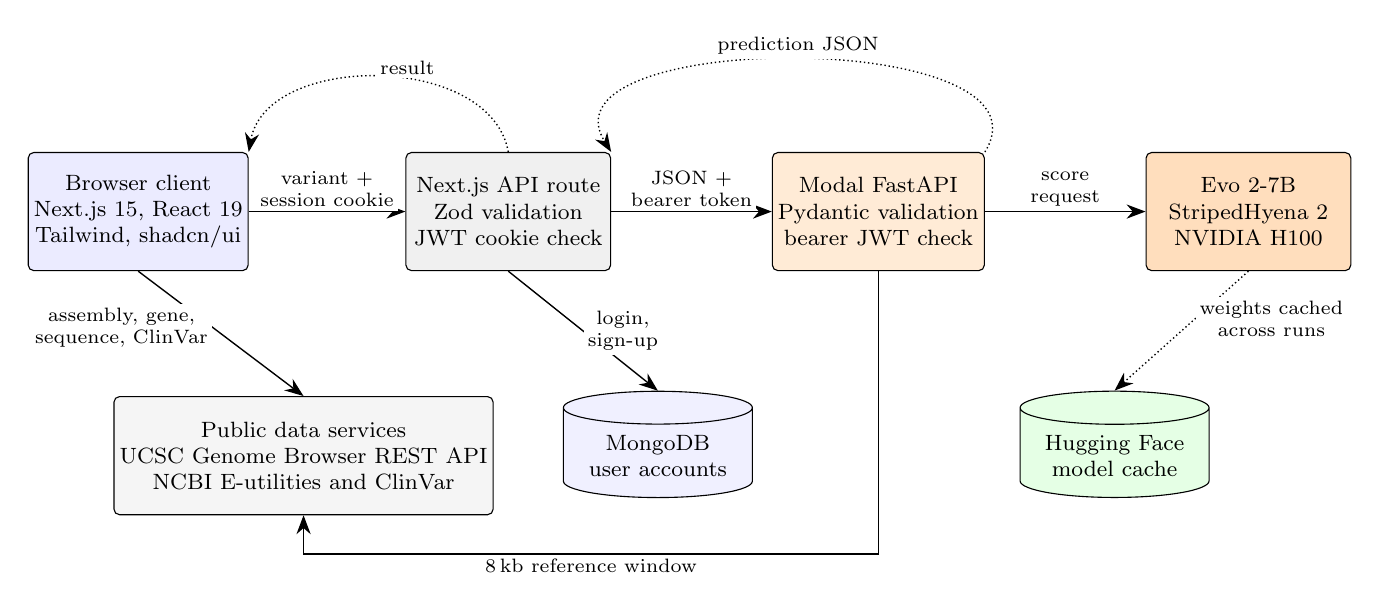
\begin{tikzpicture}[>=Stealth,font=\footnotesize,
  box/.style={rectangle,draw,rounded corners=2pt,minimum width=2.6cm,minimum height=1.5cm,align=center,inner sep=2pt,line width=0.4pt},
  store/.style={cylinder,draw,shape border rotate=90,aspect=0.22,minimum width=2.4cm,minimum height=1.35cm,align=center,inner sep=2pt,line width=0.4pt},
  lbl/.style={font=\scriptsize,align=center,inner sep=1.5pt,fill=white},
  edge/.style={-{Stealth[length=2.4mm]},line width=0.5pt},
  back/.style={-{Stealth[length=2.4mm]},line width=0.5pt,densely dotted}]
\node[box,fill=blue!8] (ui) at (0,0) {Browser client\\Next.js 15, React 19\\Tailwind, shadcn/ui};
\node[box,fill=gray!12] (route) at (4.7,0) {Next.js API route\\Zod validation\\JWT cookie check};
\node[box,fill=orange!16] (api) at (9.4,0) {Modal FastAPI\\Pydantic validation\\bearer JWT check};
\node[box,fill=orange!26] (gpu) at (14.1,0) {Evo 2-7B\\StripedHyena 2\\NVIDIA H100};
\node[store,fill=green!10] (cache) at (12.4,-3.1) {Hugging Face\\model cache};
\node[box,fill=gray!8,minimum width=4.6cm] (pub) at (2.1,-3.1) {Public data services\\UCSC Genome Browser REST API\\NCBI E-utilities and ClinVar};
\node[store,fill=blue!6] (db) at (6.6,-3.1) {MongoDB\\user accounts};
\draw[edge] (ui.east) -- node[lbl,above,pos=0.5]{variant +\\session cookie} (route.west);
\draw[edge] (route.east) -- node[lbl,above,pos=0.5]{JSON +\\bearer token} (api.west);
\draw[edge] (api.east) -- node[lbl,above,pos=0.5]{score\\request} (gpu.west);
\draw[back] (gpu.south) -- node[lbl,right,pos=0.40]{weights cached\\across runs} (cache.north);
\draw[back] (api.north east) to[out=58,in=122] node[lbl,above,pos=0.5]{prediction JSON} (route.north east);
\draw[back] (route.north) to[out=100,in=80] node[lbl,above,pos=0.42]{result} (ui.north east);
\draw[edge] (ui.south) -- node[lbl,left,pos=0.45]{assembly, gene,\\sequence, ClinVar} (pub.north);
\draw[edge] (api.south) -- (9.4,-4.35) -- node[lbl,below,pos=0.5]{8\,kb reference window} (2.1,-4.35) -- (pub.south);
\draw[edge] (route.south) -- node[lbl,right,pos=0.5]{login,\\sign-up} (db.north);
\end{tikzpicture}
\caption{System architecture. The browser performs all public data lookups and sends analysis requests to the Next.js API route, which checks the session and forwards a signed bearer token to the Modal GPU endpoint. The endpoint verifies the token, fetches an 8\,kb reference window from UCSC, scores the reference and mutated sequences with Evo~2 and returns the prediction. Solid arrows are requests; dotted arrows are responses.}
\label{fig:arch}
\end{figure*}

\subsection{Data Sources}
\begin{itemize}
\item \textbf{UCSC Genome Browser REST API}~\cite{lee2022ucsc}: list of human assemblies (hg38 by default, hg19 and others available), chromosomes, and the reference DNA sequence of any interval.
\item \textbf{NCBI Gene and E-utilities}: gene search and gene coordinates.
\item \textbf{ClinVar}~\cite{landrum2024clinvar}: known variants of the selected gene with their clinical significance, searched by position in the selected assembly.
\item \textbf{BRCA1 saturation genome editing (SGE) data}~\cite{findlay2018brca1}: experimental function scores for 3{,}893 single-nucleotide variants of \emph{BRCA1}, each labelled functional, intermediate or non-functional. This dataset is used to calibrate the decision threshold.
\end{itemize}

\subsection{Zero-Shot Scoring with Evo~2}
Evo~2 is an autoregressive language model: given a DNA sequence, it assigns a probability to every base given the bases before it. Let $S(w)$ be the mean log-likelihood per base that the model assigns to sequence $w$. A sequence that ``looks natural'' to the model receives a high $S$. A harmful mutation usually makes the sequence look less natural, so its score drops~\cite{brixi2026evo2}.

\textit{Context window.} For a variant at 1-based coordinate $p$, the backend requests from UCSC a window of about $W=8192$ bases centred on the variant, with half-width $h=W/2=4096$:
\begin{equation}
s=\max(0,\,c-1-h), \qquad e=c-1+h+1,
\label{eq:window}
\end{equation}
where the centre $c$ is $p$ for a substitution or insertion and $p+\lfloor(n-1)/2\rfloor$ for a deletion of $n$ bases, so that flanking context stays balanced. The offset of the variant inside the window is $r=p-1-s$.

\textit{Mutated sequence.} With reference window $w$, alternate base $a$, deletion length $n$ and inserted string $q$, the mutated sequence for each supported variant type is (Fig.~\ref{fig:edits})
\begin{align}
w^{\mathrm{SNV}} &= w_{0:r} + a + w_{r+1:}, \label{eq:snv}\\
w^{\mathrm{DEL}} &= w_{0:r} + w_{r+n:}, \label{eq:del}\\
w^{\mathrm{INS}} &= w_{0:r+1} + q + w_{r+1:}, \label{eq:ins}\\
w^{\mathrm{DELINS}} &= w_{0:r} + q + w_{r+n:}. \label{eq:delins}
\end{align}
Deletions and insertions are limited to 500 bases.

\begin{figure}[!t]
\centering
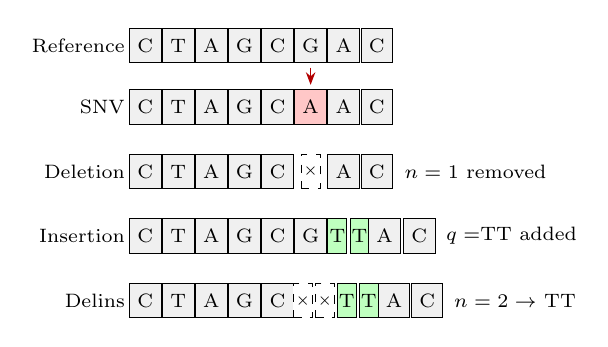
\begin{tikzpicture}[font=\scriptsize,
  cell/.style={rectangle,draw,minimum width=0.40cm,minimum height=0.44cm,align=center,inner sep=0pt,line width=0.35pt},
  ctx/.style={cell,fill=gray!12},
  altc/.style={cell,fill=red!22},
  nar/.style={rectangle,draw,minimum width=0.24cm,minimum height=0.44cm,align=center,inner sep=0pt,line width=0.35pt},
  insc/.style={nar,fill=green!25},
  gapc/.style={nar,dashed,fill=white},
  rowlbl/.style={font=\scriptsize,anchor=east,inner sep=1.5pt},
  note/.style={font=\scriptsize,anchor=west,inner sep=1pt}]
\node[rowlbl] at (-0.20,0) {Reference};
\node[ctx] at (0,0) {C};  \node[ctx] at (0.42,0) {T};
\node[ctx] at (0.84,0) {A}; \node[ctx] at (1.26,0) {G};
\node[ctx] at (1.68,0) {C}; \node[ctx] at (2.10,0) {G};
\node[ctx] at (2.52,0) {A}; \node[ctx] at (2.94,0) {C};
\node[rowlbl] at (-0.20,-0.78) {SNV};
\node[ctx] at (0,-0.78) {C};  \node[ctx] at (0.42,-0.78) {T};
\node[ctx] at (0.84,-0.78) {A}; \node[ctx] at (1.26,-0.78) {G};
\node[ctx] at (1.68,-0.78) {C}; \node[altc] at (2.10,-0.78) {A};
\node[ctx] at (2.52,-0.78) {A}; \node[ctx] at (2.94,-0.78) {C};
\draw[-{Stealth[length=1.6mm]},red!70!black,line width=0.5pt] (2.10,-0.28) -- (2.10,-0.50);
\node[rowlbl] at (-0.20,-1.60) {Deletion};
\node[ctx] at (0,-1.60) {C};  \node[ctx] at (0.42,-1.60) {T};
\node[ctx] at (0.84,-1.60) {A}; \node[ctx] at (1.26,-1.60) {G};
\node[ctx] at (1.68,-1.60) {C}; \node[gapc] at (2.10,-1.60) {\tiny$\times$};
\node[ctx] at (2.52,-1.60) {A}; \node[ctx] at (2.94,-1.60) {C};
\node[note] at (3.25,-1.60) {$n=1$ removed};
\node[rowlbl] at (-0.20,-2.42) {Insertion};
\node[ctx] at (0,-2.42) {C};  \node[ctx] at (0.42,-2.42) {T};
\node[ctx] at (0.84,-2.42) {A}; \node[ctx] at (1.26,-2.42) {G};
\node[ctx] at (1.68,-2.42) {C}; \node[ctx] at (2.10,-2.42) {G};
\node[insc] at (2.44,-2.42) {T}; \node[insc] at (2.72,-2.42) {T};
\node[ctx] at (3.04,-2.42) {A}; \node[ctx] at (3.48,-2.42) {C};
\node[note] at (3.78,-2.42) {$q=$TT added};
\node[rowlbl] at (-0.20,-3.24) {Delins};
\node[ctx] at (0,-3.24) {C};  \node[ctx] at (0.42,-3.24) {T};
\node[ctx] at (0.84,-3.24) {A}; \node[ctx] at (1.26,-3.24) {G};
\node[ctx] at (1.68,-3.24) {C};
\node[gapc] at (2.00,-3.24) {\tiny$\times$}; \node[gapc] at (2.28,-3.24) {\tiny$\times$};
\node[insc] at (2.56,-3.24) {T}; \node[insc] at (2.84,-3.24) {T};
\node[ctx] at (3.16,-3.24) {A}; \node[ctx] at (3.58,-3.24) {C};
\node[note] at (3.88,-3.24) {$n=2\rightarrow$ TT};
\end{tikzpicture}
\caption{The four mutation types supported by the backend. Context bases are grey, the substituted base red and inserted bases green; a crossed cell is a removed base.}
\label{fig:edits}
\end{figure}

\textit{Score difference.} Both sequences are scored by the model and the difference
\begin{equation}
\Delta = S(w^{\mathrm{var}}) - S(w^{\mathrm{ref}})
\label{eq:delta}
\end{equation}
is computed. A negative $\Delta$ means that the model finds the mutated sequence less likely, which suggests that the mutation is disruptive.

\subsection{Threshold Calibration}
To turn $\Delta$ into a decision, we calibrated a threshold on the BRCA1 SGE data~\cite{findlay2018brca1}, following the zero-shot protocol of the Evo~2 authors~\cite{brixi2026evo2}. Non-functional variants were treated as the positive (loss-of-function, LOF) class and functional plus intermediate variants as the negative class. For each variant we built an 8192-base window from the GRCh37 chromosome~17 sequence, scored the reference and mutated windows, and computed $\Delta$. Identical reference windows were scored only once. Because the run is costly on a single GPU, the first 500 rows of the dataset were used. The threshold $\tau$ was chosen to maximise Youden's index on the ROC curve of $-\Delta$~\cite{hanley1982roc,youden1950index}:
\begin{equation}
J(t)=\mathrm{TPR}(t)-\mathrm{FPR}(t), \qquad \tau=-\arg\max_t J(t).
\label{eq:youden}
\end{equation}
The run produced $\tau=-9.18\times10^{-4}$, and the standard deviations of $\Delta$ in the two classes were $\sigma_{\mathrm{LOF}}=1.51\times10^{-3}$ and $\sigma_{\mathrm{FUNC}}=9.02\times10^{-4}$.

\subsection{Prediction and Confidence}
The deployed endpoint labels a variant as
\begin{equation}
\mathrm{label}=\begin{cases}
\text{Likely pathogenic}, & \Delta < \tau,\\
\text{Likely benign}, & \text{otherwise},
\end{cases}
\label{eq:call}
\end{equation}
and reports a confidence value that grows with the distance of $\Delta$ from the threshold, scaled by the spread of the predicted class:
\begin{equation}
\mathrm{conf}=\min\!\left(1,\frac{|\Delta-\tau|}{\sigma_{\mathrm{class}}}\right).
\label{eq:conf}
\end{equation}
Fig.~\ref{fig:conf} plots this function. The confidence value is a heuristic distance, not a calibrated probability. Because the threshold was calibrated on substitutions, predictions for deletions, insertions and delins are flagged as \emph{provisional} in the response and the interface.

\begin{figure}[!t]
\centering
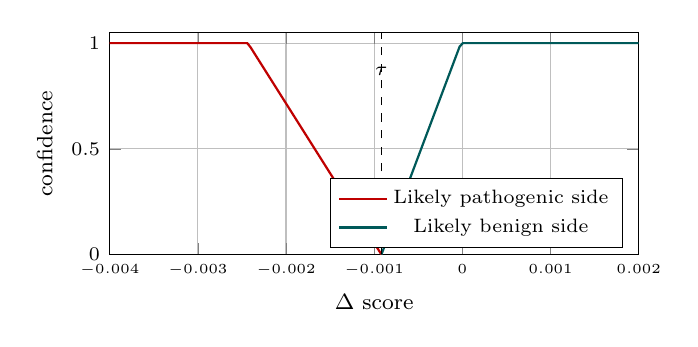
\begin{tikzpicture}
\begin{axis}[width=8.3cm,height=4.4cm,grid=major,
 xlabel={$\Delta$ score},ylabel={confidence},
 xmin=-0.004,xmax=0.002,ymin=0,ymax=1.05,
 legend pos=south east,legend style={font=\scriptsize},
 tick label style={font=\scriptsize},label style={font=\footnotesize},
 scaled x ticks=false,xtick={-0.004,-0.003,-0.002,-0.001,0,0.001,0.002},
 xticklabel style={/pgf/number format/fixed,/pgf/number format/precision=3,font=\tiny}]
\addplot[thick,red!75!black,domain=-0.004:\confTau,samples=80] {min(1,abs(x-\confTau)/\confSigLOF)};
\addplot[thick,teal!70!black,domain=\confTau:0.002,samples=80] {min(1,abs(x-\confTau)/\confSigFUNC)};
\addplot[dashed,black,line width=0.4pt] coordinates {(\confTau,0) (\confTau,1.05)};
\node[font=\scriptsize,anchor=south] at (axis cs:\confTau,0.80) {$\tau$};
\legend{Likely pathogenic side,Likely benign side}
\end{axis}
\end{tikzpicture}
\caption{The confidence function of Eq.~\eqref{eq:conf}: the distance of $\Delta$ from the threshold $\tau$, divided by the spread of the predicted class and capped at one.}
\label{fig:conf}
\end{figure}

\subsection{Security and Request Validation}
Users register and sign in with an e-mail and password; passwords are stored as bcrypt hashes in MongoDB. On sign-in, the server issues an HS256 JSON Web Token (JWT) in an HTTP-only cookie valid for seven days. The Next.js route validates every analysis request with a Zod schema and forwards it with the token as a bearer header; the Modal endpoint re-validates the request with a Pydantic model and verifies the token before using the GPU. An unauthenticated request receives HTTP~401, so the GPU cannot be used anonymously.

%% ----------------------------------------------------------------------
\section{Implementation}
\label{sec:impl}

\subsection{User Workflow}
Fig.~\ref{fig:flow} shows how a user moves through the application. After signing in, the user picks an assembly, then either browses a chromosome or searches for a gene by name. Selecting a gene shows its details, its reference sequence (up to 10{,}000 bases) and up to 20 known ClinVar variants. Clicking any base in the sequence fills the position and reference base of the variant form. The user chooses the mutation type and alternate base or sequence, and submits. For a known ClinVar variant, a single click runs Evo~2 on it and opens a comparison view that places the model's prediction next to the ClinVar classification.

\begin{figure}[!t]
\centering
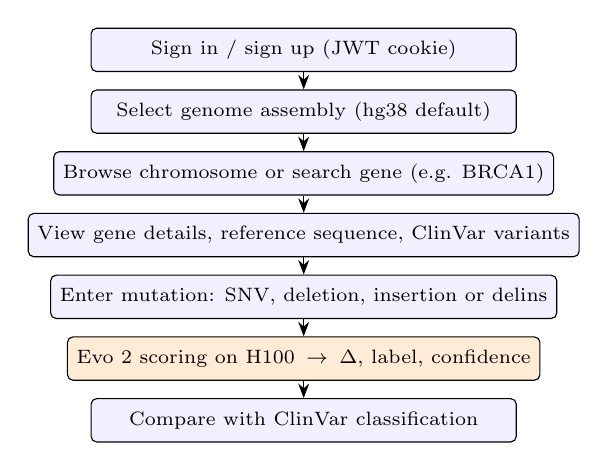
\begin{tikzpicture}[font=\scriptsize,>=Stealth,
 n/.style={rectangle,draw,rounded corners=2pt,minimum width=5.4cm,minimum height=0.55cm,align=center,fill=blue!6,line width=0.4pt},
 g/.style={n,fill=orange!16}]
\node[n] (a) {Sign in / sign up (JWT cookie)};
\node[n,below=0.22cm of a] (b) {Select genome assembly (hg38 default)};
\node[n,below=0.22cm of b] (c) {Browse chromosome or search gene (e.g. BRCA1)};
\node[n,below=0.22cm of c] (d) {View gene details, reference sequence, ClinVar variants};
\node[n,below=0.22cm of d] (e) {Enter mutation: SNV, deletion, insertion or delins};
\node[g,below=0.22cm of e] (f) {Evo 2 scoring on H100 \,$\rightarrow$\, $\Delta$, label, confidence};
\node[n,below=0.22cm of f] (h) {Compare with ClinVar classification};
\foreach \x/\y in {a/b,b/c,c/d,d/e,e/f,f/h} \draw[->,line width=0.5pt] (\x) -- (\y);
\end{tikzpicture}
\caption{User workflow of the web application.}
\label{fig:flow}
\end{figure}

\subsection{Front End}
The front end is a Next.js~15 application built on the T3 stack with React~19, TypeScript, Tailwind CSS and shadcn/ui components. All genome lookups are made from the browser to the public UCSC, NCBI clinical-tables and E-utilities services. ClinVar records are searched with the \texttt{chrpos38} field for hg38 and the \texttt{chrpos37} field for hg19. The interface colours bases, highlights the selected position, and shows the prediction as a coloured label with a confidence bar, together with the $\Delta$ score and the threshold used.

\subsection{Back End}
The back end is a Python application deployed on Modal. The container image is based on CUDA~12.6.3 with Python~3.12, PyTorch~2.7.1 and FlashAttention~2.8.0, and installs the official Evo~2 package. A persistent Hugging Face cache volume stores the model weights, so they are downloaded only once. The model is loaded when a container starts (\texttt{@modal.enter}), and the analysis function is exposed as a FastAPI POST endpoint. Modal scales the service automatically from zero to at most three H100 containers, keeps an idle container warm for 120\,s, and retries failed calls twice. The same code base contains the calibration routine of Section~\ref{sec:method}, which runs as a separate Modal GPU job. Table~\ref{tab:stack} lists the technology stack.

\begin{table}[!t]
\caption{Technology stack.}
\label{tab:stack}
\centering
\footnotesize
\begin{tabular}{@{}ll@{}}
\toprule
Layer & Technology \\
\midrule
Model & Evo 2-7B (StripedHyena 2), 8\,kb window \\
GPU serving & Modal serverless NVIDIA H100, FastAPI \\
Deep learning & PyTorch 2.7, FlashAttention 2.8, CUDA 12.6 \\
Web front end & Next.js 15, React 19, TypeScript \\
UI & Tailwind CSS 4, shadcn/ui \\
Authentication & JWT (jose, PyJWT), bcrypt, MongoDB \\
Validation & Zod (web), Pydantic (GPU tier) \\
Genome data & UCSC REST API, NCBI E-utilities, ClinVar \\
Analysis & pandas, scikit-learn, Biopython \\
\bottomrule
\end{tabular}
\end{table}

\subsection{API Contract}
A request to the endpoint is a small JSON object, for example
\begin{center}
\footnotesize
\begin{tabular}{@{}l@{}}
\texttt{\{"variant\_position": 43119628,}\\
\texttt{\ \ "variant\_type": "snv", "alternative": "G",}\\
\texttt{\ \ "genome": "hg38", "chromosome": "chr17"\}}
\end{tabular}
\end{center}
and the response contains the reference and alternate alleles, the $\Delta$ score, the label, the confidence, the threshold used and the provisional flag.

%% ----------------------------------------------------------------------
\section{Results and Discussion}
\label{sec:results}

All analysis scripts and their machine-readable outputs are included in the project repository under \texttt{docs/analysis}, so every number below except the Evo~2 calibration AUROC can be reproduced without a GPU.

\subsection{Calibration Data}
The BRCA1 workbook contains 3{,}893 variants: 2{,}821 functional (72.46\%), 249 intermediate (6.40\%) and 823 non-functional (21.14\%). This matches the published proportions of 72.5\%, 6.4\% and 21.1\%~\cite{findlay2018brca1}, confirming that the data were read correctly. All 500 reference bases of the calibration rows match the GRCh37 reference sequence.

The 500-row calibration set contains 100 non-functional and 400 functional variants, a 20.0\% positive rate close to that of the full assay. It is, however, concentrated in one part of the gene: it covers 8{,}380 of the 78{,}413 assayed bases (10.7\%), 168 distinct transcript positions and 41 amino-acid positions (Fig.~\ref{fig:slice}, Table~\ref{tab:slice}). This is the main reason why results on this set differ from results on the whole assay.

\begin{figure}[!t]
\centering
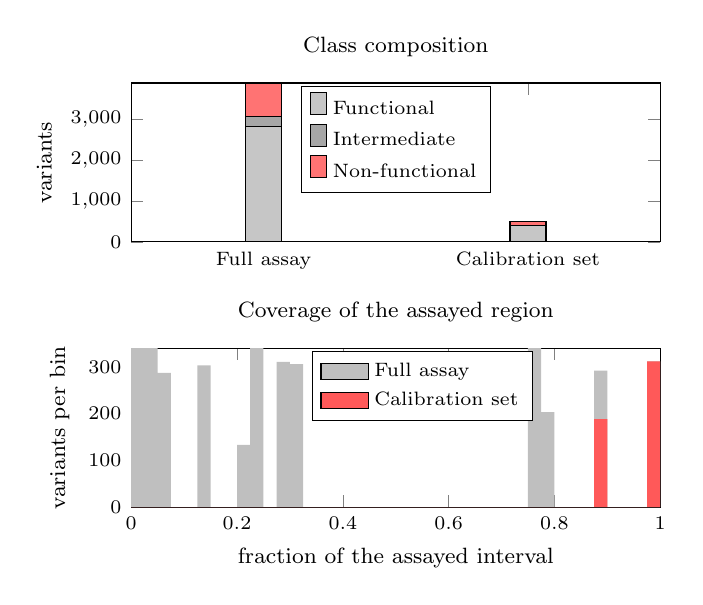
\begin{tikzpicture}
\begin{groupplot}[width=8.3cm,height=3.6cm,
 group style={group size=1 by 2, vertical sep=1.35cm},
 xlabel style={font=\footnotesize},ylabel style={font=\footnotesize},
 tick label style={font=\scriptsize},
 legend style={font=\scriptsize,at={(0.98,0.98)},anchor=north east}]
\nextgroupplot[
 title={Class composition},title style={font=\footnotesize},
 ybar stacked,bar width=13pt,
 symbolic x coords={Full assay,Calibration set},
 xtick=data,ylabel={variants},
 ymin=0,ymax=3900,enlarge x limits=0.5,legend cell align=left,
 legend style={at={(0.5,0.98)},anchor=north}]
\addplot[fill=gray!45] coordinates {(Full assay,\assayFUNC) (Calibration set,\sliceFUNC)};
\addplot[fill=gray!70] coordinates {(Full assay,\assayINT) (Calibration set,\sliceINT)};
\addplot[fill=red!55] coordinates {(Full assay,\assayLOF) (Calibration set,\sliceLOF)};
\legend{Functional,Intermediate,Non-functional}
\nextgroupplot[
 title={Coverage of the assayed region},title style={font=\footnotesize},
 xlabel={fraction of the assayed interval},ylabel={variants per bin},
 xmin=0,xmax=1,ymin=0,ymax=340,
 legend cell align={left},legend style={font=\scriptsize,at={(0.55,0.98)},anchor=north}]
\addplot[ybar interval,fill=gray!50,draw=none,mark=none,area legend] coordinates {\coverageAll};
\addplot[ybar interval,fill=red!65,draw=none,mark=none,area legend] coordinates {\coverageSlice};
\legend{Full assay,Calibration set}
\end{groupplot}
\end{tikzpicture}
\caption{The BRCA1 calibration data. Top: class composition of the full assay and of the 500-variant calibration set. Bottom: number of variants per bin along the assayed interval; the calibration set occupies two clusters at one end of the interval.}
\label{fig:slice}
\end{figure}

\begin{table}[!t]
\caption{BRCA1 data used for calibration.}
\label{tab:slice}
\centering
\footnotesize
\begin{tabular}{@{}lrr@{}}
\toprule
Property & Full assay & Calibration set \\
\midrule
Variants & 3{,}893 & 500 \\
Non-functional (LOF) & 823 (21.1\%) & 100 (20.0\%) \\
Functional + intermediate & 3{,}070 (78.9\%) & 400 (80.0\%) \\
Transcript positions & 1{,}326 & 168 \\
Amino-acid positions & 326 & 41 \\
Genomic span (GRCh37) & 78{,}413\,bp & 8{,}380\,bp \\
Reference windows scored & 1{,}326 & 168 \\
Window GC content (mean) & --- & 46.2\% \\
\bottomrule
\end{tabular}
\end{table}

\subsection{Prediction Performance}
On the 500-variant calibration set, our zero-shot Evo~2-7B run separated the two classes with an AUROC of approximately 0.73: loss-of-function variants were shifted towards more negative $\Delta$ than functional variants, and the Youden threshold of this run is $\tau=-9.18\times10^{-4}$. No fine-tuning or BRCA1-specific training was used. The detailed per-variant output of this run was not archived, so we report the AUROC to two decimals.

To put this number in context, we evaluated the predictors whose scores are included in the SGE workbook on exactly the same 500 rows, with the same labels and the same Youden procedure (Table~\ref{tab:baselines}, Fig.~\ref{fig:roc}). Confidence intervals come from 2{,}000 stratified bootstrap resamples.

\begin{table}[!t]
\caption{Predictors on the 500-variant BRCA1 calibration set. AUROC with 95\% bootstrap intervals; sensitivity and specificity at the Youden operating point. $n$: rows for which the score is available.}
\label{tab:baselines}
\centering
\footnotesize
\setlength{\tabcolsep}{4pt}
\begin{tabular}{@{}lcrrrr@{}}
\toprule
Predictor & $n$ & AUROC & 95\% CI & Sens. & Spec. \\
\midrule
Align-GVGD & 268 & 0.878 & 0.821--0.929 & 0.762 & 0.917 \\
CADD & 500 & 0.791 & 0.750--0.835 & 0.900 & 0.615 \\
phyloP & 500 & 0.777 & 0.729--0.820 & 0.880 & 0.605 \\
\textbf{Evo 2-7B (ours)} & 500 & $\approx$\textbf{0.73} & --- & --- & --- \\
PolyPhen-2 & 268 & 0.683 & 0.613--0.750 & 0.825 & 0.517 \\
SIFT & 268 & 0.656 & 0.624--0.688 & 1.000 & 0.312 \\
gnomAD AF & 500 & 0.530 & 0.506--0.553 & 0.960 & 0.100 \\
\midrule
Random & 500 & 0.500 & --- & --- & --- \\
\bottomrule
\end{tabular}
\end{table}

\begin{figure}[!t]
\centering
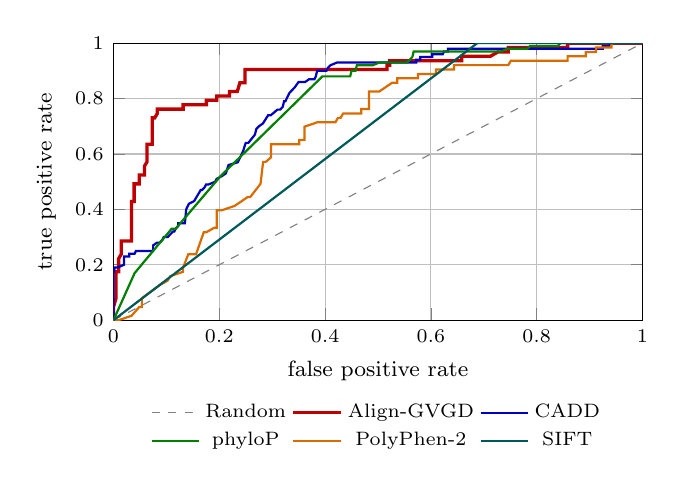
\begin{tikzpicture}
\begin{axis}[width=8.3cm,height=5.1cm,grid=major,
 xlabel={false positive rate},ylabel={true positive rate},
 xmin=0,xmax=1,ymin=0,ymax=1,
 legend style={font=\scriptsize,at={(0.5,-0.26)},anchor=north,legend columns=3,draw=none},
 tick label style={font=\scriptsize},label style={font=\footnotesize}]
\addplot[dashed,gray,line width=0.4pt] coordinates {(0,0) (1,1)};
\addplot[very thick,red!75!black] coordinates {\rocaGVD};
\addplot[thick,blue!75!black] coordinates {\rocCADD};
\addplot[thick,green!50!black] coordinates {\rocphyloP};
\addplot[thick,orange!85!black] coordinates {\rocPolyPhen2};
\addplot[thick,teal!70!black] coordinates {\rocSIFT};
\legend{Random,Align-GVGD,CADD,phyloP,PolyPhen-2,SIFT}
\end{axis}
\end{tikzpicture}
\caption{ROC curves of the reference predictors on the 500-variant calibration set, with loss-of-function as the positive class.}
\label{fig:roc}
\end{figure}

Three observations follow. First, the calibration set is harder than the full assay for every predictor: CADD falls from 0.876 on all 3{,}893 variants~\cite{brixi2026evo2} to 0.791 here, so the drop of Evo~2 from the published 0.904 to about 0.73 is consistent with the composition of the set rather than with a fault in the pipeline. Second, on these rows Evo~2 is clearly better than chance, SIFT, PolyPhen-2 and population frequency, but below CADD, phyloP and Align-GVGD, which use alignments and annotations that Evo~2 does not see. Third, the bootstrap intervals are up to about $\pm0.05$ wide, so small differences between neighbouring predictors are not significant on 500 variants. Table~\ref{tab:evo2} lists the published results on the full assay for comparison.

\begin{table}[!t]
\caption{Published zero-shot results on the full BRCA1 assay (3{,}893 variants)~\cite{brixi2026evo2}, for reference.}
\label{tab:evo2}
\centering
\footnotesize
\begin{tabular}{@{}lrr@{}}
\toprule
Model & AUROC & AUPRC \\
\midrule
Evo 2-7B & 0.904 & 0.733 \\
Evo 2-40B & 0.901 & 0.677 \\
CADD & 0.876 & 0.730 \\
GPN-MSA & 0.863 & 0.650 \\
phyloP (100 vertebrates) & 0.811 & 0.495 \\
Nucleotide Transformer & 0.550 & 0.285 \\
Evo 1 & 0.497 & 0.216 \\
\bottomrule
\end{tabular}
\end{table}

\subsection{System Functionality}
The deployed system was demonstrated end to end with the example request of Section~\ref{sec:impl} (hg38, chr17:43{,}119{,}628, alternate G) and with known BRCA1 variants selected from the ClinVar table. In each case the endpoint fetched the window and the reference base from UCSC and returned the $\Delta$ score, label, confidence and threshold, which the interface displayed beside the ClinVar classification. Both tiers are coded to reject unauthenticated requests with HTTP~401. The scoring code was also checked offline with a simple stand-in scorer in place of Evo~2: a 3-base deletion produced sequences of 8{,}193 and 8{,}190 bases and a 3-base insertion 8{,}193 and 8{,}196 bases, as Eqs.~\eqref{eq:del}--\eqref{eq:ins} require. Two forward passes over about 8{,}200 bases are needed per request. We have not yet benchmarked latency or throughput.

\subsection{Verification of the Deployed Pipeline}
Because a prediction is only as good as the coordinate and sequence it is computed on, we verified the pipeline itself.

\textit{Context window.} Over all 500 calibration positions, the deployed window (Eq.~\eqref{eq:window}) is identical to the calibration window except for one extra base at the 3$'$ end (8{,}193 versus 8{,}192 bases). The variant sits at the same offset, 4{,}096, in both. The effect on $\Delta$ is expected to be small, but the two should be aligned.

\textit{Genome assembly.} The threshold was calibrated on GRCh37 (hg19) coordinates, whereas the interface defaults to GRCh38 (hg38). Aligning the two assemblies over \emph{BRCA1} gives a constant offset of 1{,}847{,}983 bases, confirmed against 290 live ClinVar records that carry both coordinates. Because the sequence of \emph{BRCA1} is identical in both assemblies across the scoring window, a correct hg38 coordinate scores exactly the intended sequence. An hg19 coordinate typed while hg38 is selected, however, points to a different base for all 500 calibration variants, and the system cannot detect this because the request does not carry the expected reference allele. We also found that the ClinVar ``analyse'' shortcut always forwards the GRCh38 position, even when hg19 is selected.

\textit{Request validation.} We generated 55 test requests covering every field, every numeric boundary, the 500-base length limit and malformed values. The Zod (web) layer handled 47 correctly and the Pydantic (GPU) layer 43; the two layers disagreed on 6 cases, all of which are rejected by the web tier before reaching the GPU. Both layers also mishandled seven cases: six assembly or chromosome strings containing characters such as ``;'' were accepted although they should be rejected before being placed in the UCSC query, and one whitespace-padded alternate base was rejected by both although the specification accepts it.

\textit{Scoring edge case.} A substitution that does not change the base produces $\Delta=0$, which Eq.~\eqref{eq:conf} reports as ``likely benign'' with confidence 1.0. Such requests should be rejected.

Table~\ref{tab:fixes} lists these findings and the corresponding improvements, which form the first part of our future work.

\begin{table}[!t]
\caption{Findings of the verification study and planned improvements.}
\label{tab:fixes}
\centering
\footnotesize
\begin{tabular}{@{}p{3.6cm}p{4.2cm}@{}}
\toprule
Finding & Improvement \\
\midrule
Request has no reference allele & Send expected reference base; reject mismatches \\
Unchanged-base SNV gets conf.\ 1.0 & Reject when alternate equals reference \\
hg19 threshold used for hg38 & Recalibrate on hg38 coordinates \\
ClinVar shortcut sends GRCh38 position & Use position of selected assembly \\
Window 8{,}193 vs.\ 8{,}192 bases & Use one window rule everywhere \\
Two validators differ on 6/55 cases & Generate both from one schema \\
Unsafe characters in assembly field & Whitelist assembly and chromosome names \\
Reference scored on every request & Cache reference scores per window \\
\bottomrule
\end{tabular}
\end{table}

%% ----------------------------------------------------------------------
\section{Applications and Societal Relevance}
\label{sec:apps}

\begin{itemize}
\item \textbf{Education.} Students of biotechnology, medicine and computer science can explore real genes, real ClinVar records and a state-of-the-art AI model from a browser, without programming or owning a GPU.
\item \textbf{Research triage.} Researchers can obtain a quick, model-based second opinion on rare or novel variants and prioritise them for laboratory follow-up.
\item \textbf{Support for genetic counselling.} By showing a model score next to the expert ClinVar classification, the tool can help counsellors and clinicians explain how computational evidence fits into the ACMG/AMP framework~\cite{richards2015acmg}, while making clear that it is only supporting evidence.
\item \textbf{Low-cost access.} Serverless GPUs are billed only while a request is being processed and scale down to zero when idle, so a college, start-up or small laboratory can host such a tool without buying GPU hardware.
\item \textbf{Extensibility.} The same pipeline can be applied to other disease genes and, with suitable calibration data, to genes of interest to Indian populations, which are under-represented in current variant databases~\cite{pathak2024ancestry}.
\end{itemize}

%% ----------------------------------------------------------------------
\section{Limitations and Future Scope}
\label{sec:limits}

\textbf{Limitations.} (i) The system is a research and teaching tool; its labels are computational predictions and must not be used for diagnosis. Under the ACMG/AMP guidelines, computational evidence can only support a classification~\cite{richards2015acmg,pejaver2022svi}. (ii) The threshold was calibrated on 500 substitutions in one region of one gene; it may not transfer to other genes, other regions, or to deletions and insertions, whose predictions are marked provisional. (iii) The confidence value is a heuristic, not a probability. (iv) The calibration AUROC comes from a single run whose per-variant output was not archived. (v) Public API limits restrict the interface to 20 ClinVar records and 10{,}000 displayed bases per gene. (vi) Language models trained on sequence alone can reflect evolutionary and ancestry biases~\cite{pugh2025likelihood,pathak2024ancestry}.

\textbf{Future scope.}
\begin{enumerate}
\item Implement the improvements in Table~\ref{tab:fixes}, starting with reference-allele checking.
\item Recalibrate on all 3{,}893 BRCA1 variants with a held-out test split and under hg38 coordinates, and report a calibrated probability (e.g.\ following ClinGen recommendations~\cite{pejaver2022svi}) instead of the heuristic confidence.
\item Calibrate separate thresholds for deletions and insertions and for other genes such as \emph{BRCA2}.
\item Add batch analysis of VCF files, result export, and caching of reference scores to reduce GPU cost.
\item Benchmark latency and cost, and evaluate the larger Evo~2-40B model.
\item Add multilingual (Kannada and English) explanations for educational use.
\end{enumerate}

%% ----------------------------------------------------------------------
\section{Conclusion}
\label{sec:conclusion}

We designed and implemented a web application that makes the Evo~2 genomic language model usable from a browser for analysing genetic mutations and their likely disease impact. The system combines public genome and ClinVar data with a serverless H100 GPU endpoint, supports four mutation types, secures the GPU behind token authentication, and places each prediction next to the expert ClinVar classification. On 500 BRCA1 variants with experimental labels, the zero-shot predictor separated harmful from harmless variants with an AUROC of about 0.73, and we placed this result alongside established predictors evaluated on the same rows. A verification study of the deployed pipeline identified eight specific improvements, the most important being to check the reference allele of every request and to recalibrate the threshold on the full dataset in hg38 coordinates. The project shows that state-of-the-art genomic AI can be made accessible to students and researchers at low cost, provided that its outputs are presented as research evidence and not as a clinical diagnosis.

\section*{Acknowledgment}
The authors thank the Karnataka State Council for Science and Technology (KSCST) for the Student Project Programme, their project guide and the Department of Artificial Intelligence and Data Science, Don Bosco Institute of Technology, for guidance and support, and the Arc Institute for releasing Evo~2 openly.

%% ----------------------------------------------------------------------
\begin{thebibliography}{00}

\bibitem{findlay2018brca1} G. M. Findlay, R. M. Daza, B. Martin, M. D. Zhang, A. P. Leith, M. Gasperini, \emph{et al.}, ``Accurate classification of \emph{BRCA1} variants with saturation genome editing,'' \textit{Nature}, vol. 562, no. 7726, pp. 217--222, 2018, doi: 10.1038/s41586-018-0461-z.

\bibitem{richards2015acmg} S. Richards, N. Aziz, S. Bale, D. Bick, S. Das, J. Gastier-Foster, \emph{et al.}, ``Standards and guidelines for the interpretation of sequence variants: a joint consensus recommendation of the American College of Medical Genetics and Genomics and the Association for Molecular Pathology,'' \textit{Genet. Med.}, vol. 17, no. 5, pp. 405--424, 2015, doi: 10.1038/gim.2015.30.

\bibitem{ng2001sift} P. C. Ng and S. Henikoff, ``Predicting deleterious amino acid substitutions,'' \textit{Genome Res.}, vol. 11, no. 5, pp. 863--874, 2001, doi: 10.1101/gr.176601.

\bibitem{adzhubei2010polyphen2} I. A. Adzhubei, S. Schmidt, L. Peshkin, V. E. Ramensky, A. Gerasimova, \emph{et al.}, ``A method and server for predicting damaging missense mutations,'' \textit{Nat. Methods}, vol. 7, no. 4, pp. 248--249, 2010, doi: 10.1038/nmeth0410-248.

\bibitem{rentzsch2019cadd} P. Rentzsch, D. Witten, G. M. Cooper, J. Shendure, and M. Kircher, ``CADD: predicting the deleteriousness of variants throughout the human genome,'' \textit{Nucleic Acids Res.}, vol. 47, no. D1, pp. D886--D894, 2019, doi: 10.1093/nar/gky1016.

\bibitem{schubach2024cadd} M. Schubach, T. Maass, L. Nazaretyan, S. R\"oner, and M. Kircher, ``CADD v1.7: using protein language models, regulatory CNNs and other nucleotide-level scores to improve genome-wide variant predictions,'' \textit{Nucleic Acids Res.}, vol. 52, no. D1, pp. D1143--D1154, 2024, doi: 10.1093/nar/gkad989.

\bibitem{brixi2026evo2} G. Brixi, M. G. Durrant, J. Ku, M. Naghipourfar, M. Poli, G. Sun, \emph{et al.}, ``Genome modelling and design across all domains of life with Evo 2,'' \textit{Nature}, 2026, doi: 10.1038/s41586-026-10176-5.

\bibitem{brixi2025stripedhyena2} J. Ku, E. Nguyen, D. W. Romero, G. Brixi, B. Yang, A. Vorontsov, \emph{et al.}, ``Systems and algorithms for convolutional multi-hybrid language models at scale,'' arXiv:2503.01868, 2025.

\bibitem{mclaren2016vep} W. McLaren, L. Gil, S. E. Hunt, H. S. Riat, G. R. S. Ritchie, A. Thormann, P. Flicek, and F. Cunningham, ``The Ensembl Variant Effect Predictor,'' \textit{Genome Biol.}, vol. 17, p. 122, 2016, doi: 10.1186/s13059-016-0974-4.

\bibitem{avsec2021enformer} \v{Z}. Avsec, V. Agarwal, D. Visentin, J. R. Ledsam, A. Grabska-Barwinska, \emph{et al.}, ``Effective gene expression prediction from sequence by integrating long-range interactions,'' \textit{Nat. Methods}, vol. 18, pp. 1196--1203, 2021, doi: 10.1038/s41592-021-01252-x.

\bibitem{linder2025borzoi} J. Linder, D. Srivastava, H. Yuan, V. Agarwal, and D. R. Kelley, ``Predicting RNA-seq coverage from DNA sequence as a unifying model of gene regulation,'' \textit{Nat. Genet.}, vol. 57, pp. 949--961, 2025, doi: 10.1038/s41588-024-02053-6.

\bibitem{lin2023esm2} Z. Lin, H. Akin, R. Rao, B. Hie, Z. Zhu, W. Lu, \emph{et al.}, ``Evolutionary-scale prediction of atomic-level protein structure with a language model,'' \textit{Science}, vol. 379, no. 6637, pp. 1123--1130, 2023, doi: 10.1126/science.ade2574.

\bibitem{cheng2023alphamissense} J. Cheng, G. Novati, J. Pan, C. Bycroft, A. \v{Z}emgulyt\.{e}, \emph{et al.}, ``Accurate proteome-wide missense variant effect prediction with AlphaMissense,'' \textit{Science}, vol. 381, no. 6664, eadg7492, 2023, doi: 10.1126/science.adg7492.

\bibitem{zhou2024dnabert2} Z. Zhou, Y. Ji, W. Li, P. Dutta, R. Davuluri, and H. Liu, ``DNABERT-2: efficient foundation model and benchmark for multi-species genomes,'' in \textit{Proc. Int. Conf. Learning Representations (ICLR)}, 2024.

\bibitem{dallatorre2024nt} H. Dalla-Torre, L. Gonzalez, J. Mendoza-Revilla, N. Lopez Carranza, \emph{et al.}, ``Nucleotide Transformer: building and evaluating robust foundation models for human genomics,'' \textit{Nat. Methods}, vol. 22, pp. 287--297, 2025, doi: 10.1038/s41592-024-02523-z.

\bibitem{benegas2025gpnmsa} G. Benegas, C. Albors, A. J. Aw, C. Ye, and Y. S. Song, ``A DNA language model based on multispecies alignment predicts the effects of genome-wide variants,'' \textit{Nat. Biotechnol.}, 2025, doi: 10.1038/s41587-024-02511-w.

\bibitem{nguyen2024evo} E. Nguyen, M. Poli, M. G. Durrant, B. Kang, D. Katrekar, \emph{et al.}, ``Sequence modeling and design from molecular to genome scale with Evo,'' \textit{Science}, vol. 386, no. 6723, eado9336, 2024, doi: 10.1126/science.ado9336.

\bibitem{vandenbroucke2019varsome} C. Kopanos, V. Tsiolkas, A. Kouris, C. E. Chapple, M. Albarca Aguilera, R. Meyer, and A. Massouras, ``VarSome: the human genomic variant search engine,'' \textit{Bioinformatics}, vol. 35, no. 11, pp. 1978--1980, 2019, doi: 10.1093/bioinformatics/bty897.

\bibitem{baux2021mobidetails} D. Baux, C. Van Goethem, O. Ardouin, T. Guignard, A. Bergougnoux, M. Koenig, and A.-F. Roux, ``MobiDetails: online DNA variants interpretation,'' \textit{Eur. J. Hum. Genet.}, vol. 29, pp. 356--360, 2021, doi: 10.1038/s41431-020-00755-z.

\bibitem{lee2022ucsc} B. T. Lee, G. P. Barber, A. Benet-Pag\`es, J. Casper, H. Clawson, M. Diekhans, \emph{et al.}, ``The UCSC Genome Browser database: 2022 update,'' \textit{Nucleic Acids Res.}, vol. 50, no. D1, pp. D1115--D1122, 2022, doi: 10.1093/nar/gkab959.

\bibitem{landrum2024clinvar} M. J. Landrum, S. Chitipiralla, K. Kaur, G. Brown, C. Chen, J. Hart, \emph{et al.}, ``ClinVar: updates to support classifications of both germline and somatic variants,'' \textit{Nucleic Acids Res.}, vol. 53, no. D1, pp. D1313--D1321, 2025, doi: 10.1093/nar/gkae1090.

\bibitem{hanley1982roc} J. A. Hanley and B. J. McNeil, ``The meaning and use of the area under a receiver operating characteristic (ROC) curve,'' \textit{Radiology}, vol. 143, no. 1, pp. 29--36, 1982.

\bibitem{youden1950index} W. J. Youden, ``Index for rating diagnostic tests,'' \textit{Cancer}, vol. 3, no. 1, pp. 32--35, 1950.

\bibitem{pejaver2022svi} V. Pejaver, A. B. Byrne, B.-J. Feng, K. A. Pagel, S. D. Mooney, R. Karchin, \emph{et al.}, ``Calibration of computational tools for missense variant pathogenicity classification and ClinGen recommendations for PP3/BP4 criteria,'' \textit{Am. J. Hum. Genet.}, vol. 109, no. 12, pp. 2163--2177, 2022, doi: 10.1016/j.ajhg.2022.10.013.

\bibitem{pugh2025likelihood} C. W. J. Pugh, P. G. Nu\~nez-Valencia, M. Dias, and J. Frazer, ``From likelihood to fitness: improving variant effect prediction in protein and genome language models,'' in \textit{Proc. NeurIPS}, 2025.

\bibitem{pathak2024ancestry} A. K. Pathak, N. Bora, M. Badonyi, B. J. Livesey, J. Ngeow, and J. A. Marsh, ``Pervasive ancestry bias in variant effect predictors,'' \textit{bioRxiv}, 2024, doi: 10.1101/2024.05.20.594987.

\end{thebibliography}

\end{document}
